\documentclass[11pt]{article}

\usepackage[margin=1in]{geometry}
\usepackage[T1]{fontenc}
\usepackage{lmodern}
\usepackage{microtype}
\usepackage{amsmath,amssymb,amsthm,mathtools}
\usepackage{mathrsfs}
\usepackage[dvipsnames]{xcolor}
\usepackage[most]{tcolorbox}
\usepackage{graphicx}
\graphicspath{{figures/}{notes/figures/}}
\usepackage{tikz}
\usetikzlibrary{decorations.markings,patterns}
\usepackage{pgfplots}
\pgfplotsset{compat=1.17}
\usepackage{enumitem}
\usepackage{tocloft}
\usepackage[hidelinks]{hyperref}

\definecolor{courseblue}{HTML}{1F4E79}
\definecolor{lightblue}{HTML}{EAF2F8}
\definecolor{lightgreen}{HTML}{EAF7EA}
\definecolor{lightpink}{HTML}{FCE8EF}
\definecolor{lightyellow}{HTML}{FFF8D6}
\definecolor{warningyellow}{HTML}{D6A000}
\definecolor{exercisebg}{HTML}{FDEAEA}
\definecolor{exerciseframe}{HTML}{B54040}
\definecolor{examplebg}{HTML}{F4FAFE}
\definecolor{exampleframe}{HTML}{85C1E9}
\definecolor{darkgray}{HTML}{333333}
\definecolor{lightorange}{HTML}{FDEBD8}
\definecolor{orangeframe}{HTML}{E08A3C}
\definecolor{remarkbg}{HTML}{F3EEFB}
\definecolor{remarkframe}{HTML}{9B7FC9}
\definecolor{cayleyred}{HTML}{C0392B}
\definecolor{cayleygreen}{HTML}{1E8449}
\definecolor{cayleyblue}{HTML}{1F5FA0}
\definecolor{cayleyorange}{HTML}{D35400}
\definecolor{cayleypurple}{HTML}{7D3C98}
\definecolor{cayleyteal}{HTML}{117A65}

\setlength{\parindent}{0pt}
\setlength{\parskip}{0.45em}
\setlist[itemize]{topsep=0.25em,itemsep=0.15em}
\renewcommand{\cftsecleader}{\cftdotfill{\cftdotsep}}
\renewcommand{\cftsubsecleader}{\cftdotfill{\cftdotsep}}

\theoremstyle{plain}
\newtheorem{theorem}{Theorem}[section]
\newtheorem{proposition}[theorem]{Proposition}
\newtheorem{lemma}[theorem]{Lemma}
\newtheorem{corollary}[theorem]{Corollary}
\theoremstyle{definition}
\newtheorem{definition}[theorem]{Definition}
\newtheorem{example}[theorem]{Example}
\newtheorem{exercise}[theorem]{Exercise}
\newtheoremstyle{boldremark}
  {3pt}{3pt}{\normalfont}{}{\bfseries}{.}{.5em}
  {\thmname{#1}\thmnumber{ #2}\thmnote{ (#3)}}
\theoremstyle{boldremark}
\newtheorem*{remark}{Remark}
\theoremstyle{remark}
\newtheorem*{fact}{Fact}
\newtheorem*{warning}{Warning}

\tcolorboxenvironment{definition}{
  enhanced,
  unbreakable,
  colback=lightgreen,
  colframe=ForestGreen,
  boxrule=0.7pt,
  arc=2pt,
  left=6pt,
  right=6pt,
  top=5pt,
  bottom=5pt
}

\tcolorboxenvironment{remark}{
  enhanced,
  colback=remarkbg,
  colframe=remarkframe,
  before upper={\setlength{\parskip}{0.5em}},
  boxrule=0.7pt,
  arc=2pt,
  left=6pt,
  right=6pt,
  top=5pt,
  bottom=5pt
}

\tcolorboxenvironment{warning}{
  enhanced,
  colback=lightyellow,
  colframe=warningyellow,
  boxrule=0.7pt,
  arc=2pt,
  left=6pt,
  right=6pt,
  top=5pt,
  bottom=5pt
}

\tcolorboxenvironment{exercise}{
  enhanced,
  unbreakable,
  colback=exercisebg,
  colframe=exerciseframe,
  boxrule=1pt,
  arc=2pt,
  left=6pt,
  right=6pt,
  top=5pt,
  bottom=5pt
}

\tcolorboxenvironment{example}{
  enhanced,
  colback=examplebg,
  colframe=exampleframe,
  boxrule=0.7pt,
  arc=2pt,
  left=6pt,
  right=6pt,
  top=5pt,
  bottom=5pt
}

\numberwithin{equation}{section}

\newcommand{\be}{\begin{eqnarray}}
\newcommand{\ee}{\end{eqnarray}}
\newcommand{\C}{\mathbb{C}}
\newcommand{\R}{\mathbb{R}}
\newcommand{\N}{\mathbb{N}}
\newcommand{\Z}{\mathbb{Z}}
\DeclareMathOperator{\Log}{Log}
\DeclareMathOperator{\Arg}{Arg}

\DeclareMathOperator{\Hol}{\mathcal{H}\mathrm{ol}}
\DeclareMathOperator{\Real}{Re}
\DeclareMathOperator{\Imag}{Im}
\newcommand{\A}{\mathcal{A}}
\newcommand{\CT}{\C[[T]]}
\newcommand{\CLT}{\C((T))}
\tcbset{breakable}
% Compact spacing around diagrams; keep the main text at 11pt.
\newenvironment{lecturefigure}
 {\par\addvspace{0.25em}\begingroup\setlength{\parskip}{0pt}\centering}
 {\par\endgroup\addvspace{0.25em}}
\begin{document}

\begin{center}
  \colorbox{lightblue}{%
    \begin{minipage}{0.94\textwidth}
      \vspace{0.55em}
      \begin{tabular*}{\textwidth}{@{\extracolsep{\fill}}lr}
        {\color{courseblue}\bfseries\LARGE Lecture 33} &
        {\color{courseblue}\bfseries\LARGE MATH 411}\\[0.35em]
        \textbf{Fall 2026} & \textbf{Date: Dec 4, 2026}\\
        & \textbf{Instructor: Manish Patnaik}
      \end{tabular*}
      \vspace{0.45em}
    \end{minipage}}
\end{center}

\setcounter{tocdepth}{1}
\tableofcontents
\vspace{0.45em}

% Source: handwritten Lecture 32, Dec. 5, pp. 1--4.
\section{Analytic continuation and functional equation of \texorpdfstring{$\zeta(s)$}{zeta(s)}}

Let us briefly collect the three special functions we have assembled over
Lectures~31 and~32:
\begin{itemize}
 \item \textbf{The theta function:} For $u>0$,
       $\Theta(u)=\sum_{n\in\Z} e^{-\pi n^2 u}$ satisfies the theta
       inversion formula $\Theta(u)=u^{-1/2}\Theta(1/u)$ (coming from
       Poisson summation) together with the decay bound
       $0<\Theta(u)-1\leq Ce^{-\pi u}$ for $u\geq 1$.
 \item \textbf{The Gamma function:} For $\Real s>0$,
       $\Gamma(s)=\int_0^{\infty} e^{-t}t^s\,\frac{dt}{t}$ is a
       \emph{Mellin transform} $\mathcal M(\varphi)(s)=\int_0^{\infty}\varphi(t)t^s\,\frac{dt}{t}$
       with $\varphi(t)=e^{-t}$. Using $s(s+1)\cdots(s+n)\Gamma(s)=\Gamma(s+n+1)$,
       $\Gamma$ continues meromorphically to $\C$ with simple poles at
       $s=0,-1,-2,\dots$; by Euler's reflection formula, $1/\Gamma(s)$ is
       entire with simple zeros precisely at $s=0,-1,-2,\dots$.
 \item \textbf{The Riemann zeta function:} For $\Real s>1$,
       $\zeta(s)=\sum_{n=1}^{\infty} n^{-s}=\prod_{p\text{ prime}}(1-p^{-s})^{-1}$
       is holomorphic.
\end{itemize}

We now prove the Mellin transform identity linking $\Theta$, $\Gamma$, and
$\zeta$, and use it to obtain the meromorphic continuation and functional
equation of $\zeta(s)$.

\begin{proposition}[Mellin transform representation]\label{prop:mellin-proof}
For every $s\in\C$ with $\Real s > 1$,
\begin{equation}\label{eq:mellin-id}
 \boxed{\displaystyle
  \pi^{-s/2}\,\Gamma\!\left(\frac{s}{2}\right)\zeta(s)
  = \frac{1}{2}\int_0^{\infty} u^{s/2-1}\bigl(\Theta(u)-1\bigr)\,du.}
\end{equation}
\end{proposition}

\begin{proof}
Recall that $\frac{1}{2}\bigl(\Theta(u)-1\bigr)=\sum_{n=1}^{\infty} e^{-\pi n^2 u}$.
Consider a single term of the integral on the right-hand side for a fixed
integer $n\geq 1$. Substituting $t=\pi n^2 u$ (so $u=t/(\pi n^2)$ and
$\frac{du}{u}=\frac{dt}{t}$) gives
\begin{align*}
 \int_0^{\infty} u^{s/2} e^{-\pi n^2 u}\,\frac{du}{u}
 &= \frac{1}{(\pi n^2)^{s/2}}\int_0^{\infty} e^{-t} t^{s/2-1}\,dt \\
 &= \pi^{-s/2}\frac{1}{n^s}\,\Gamma\!\left(\frac{s}{2}\right).
\end{align*}
Because $\sigma=\Real s > 1$, the sum of the integrals of the absolute
values converges:
\[
 \sum_{n=1}^{\infty}\int_0^{\infty}\bigl|u^{s/2-1}e^{-\pi n^2 u}\bigr|\,du
 = \sum_{n=1}^{\infty}\int_0^{\infty} u^{\sigma/2-1}e^{-\pi n^2 u}\,du
 = \pi^{-\sigma/2}\,\Gamma\!\left(\frac{\sigma}{2}\right)\sum_{n=1}^{\infty}\frac{1}{n^{\sigma}}
 < \infty.
\]
We may therefore interchange summation and integration:
\[
 \frac{1}{2}\int_0^{\infty} u^{s/2-1}\bigl(\Theta(u)-1\bigr)\,du
 = \sum_{n=1}^{\infty}\int_0^{\infty} u^{s/2-1}e^{-\pi n^2 u}\,du
 = \pi^{-s/2}\,\Gamma\!\left(\frac{s}{2}\right)\sum_{n=1}^{\infty}\frac{1}{n^s}
 = \pi^{-s/2}\,\Gamma\!\left(\frac{s}{2}\right)\zeta(s). \qedhere
\]
\end{proof}

It is convenient to name the left-hand side of \eqref{eq:mellin-id}. Define
the \emph{completed zeta function}
\[
 \xi(s) = \pi^{-s/2}\,\Gamma\!\left(\frac{s}{2}\right)\zeta(s)
 \qquad (\Real s > 1).
\]

\begin{theorem}[Continuation and functional equation of $\xi(s)$]\label{thm:xi-cont}
\leavevmode
\begin{enumerate}[label=\textup{(\arabic*)}]
 \item The function $\xi(s)$ has an analytic continuation to all of $\C$ as
       a meromorphic function whose only poles are simple poles at $s=0$
       and $s=1$.
 \item For all $s\in\C\setminus\{0,1\}$, $\xi(s)$ satisfies the
       \emph{functional equation}
       \begin{equation}\label{eq:func-eq}
        \boxed{\displaystyle \xi(s) = \xi(1-s).}
       \end{equation}
\end{enumerate}
\end{theorem}

\begin{proof}
Set $\phi(u)=\frac{\Theta(u)-1}{2}=\sum_{n=1}^{\infty} e^{-\pi n^2 u}$ for
$u>0$, so $\Theta(u)=2\phi(u)+1$. Substituting this into the theta
inversion formula $\Theta(u)=u^{-1/2}\Theta(1/u)$ gives
\[
 2\phi(u)+1 = u^{-1/2}\bigl(2\phi(1/u)+1\bigr),
\]
and hence
\begin{equation}\label{eq:phi-inv}
 \boxed{\displaystyle
  \phi(u) = u^{-1/2}\phi\!\left(\frac{1}{u}\right) + \frac{1}{2u^{1/2}} - \frac{1}{2}.}
\end{equation}

Now take $\Real s > 1$. By Proposition~\ref{prop:mellin-proof}, split the
integral defining $\xi(s)$ at $u=1$:
\[
 \xi(s) = \int_0^{\infty} u^{s/2-1}\phi(u)\,du
        = \int_0^{1} u^{s/2-1}\phi(u)\,du
        + \int_1^{\infty} u^{s/2-1}\phi(u)\,du.
\]
Substitute \eqref{eq:phi-inv} into the integral over $(0,1]$:
\[
 \int_0^{1} u^{s/2-1}\phi(u)\,du
 = \int_0^{1} u^{s/2-1}
   \left[u^{-1/2}\phi\!\left(\frac{1}{u}\right)
         + \frac{1}{2u^{1/2}} - \frac{1}{2}\right]du.
\]
For $\Real s > 1$, the elementary part evaluates directly:
\[
 \int_0^{1}\left(\frac{1}{2}u^{(s-1)/2-1} - \frac{1}{2}u^{s/2-1}\right)du
 = \left[\frac{u^{(s-1)/2}}{s-1} - \frac{u^{s/2}}{s}\right]_0^1
 = \frac{1}{s-1} - \frac{1}{s},
\]
since $\Real((s-1)/2)>0$ and $\Real(s/2)>1/2>0$. For the remaining integral
over $(0,1]$, change variables via $v=1/u$ ($u=1/v$, $du=-v^{-2}\,dv$):
\[
 \int_0^{1} u^{s/2-3/2}\phi\!\left(\frac{1}{u}\right)du
 = \int_{\infty}^{1} v^{-s/2+3/2}\phi(v)\bigl(-v^{-2}\,dv\bigr)
 = \int_1^{\infty} v^{-s/2-1/2}\phi(v)\,dv.
\]
Relabeling $v$ as $u$ and combining with the integral over $[1,\infty)$, we
obtain, for all $\Real s > 1$,
\begin{equation}\label{eq:xi-global}
 \xi(s) = \underbrace{\frac{1}{s-1} - \frac{1}{s}}_{\substack{\text{meromorphic,}\\\text{poles at }s=0,1}}
        + \underbrace{\int_1^{\infty}
          \bigl(u^{-s/2-1/2} + u^{s/2-1}\bigr)\phi(u)\,du}_{\text{entire on }\C}.
\end{equation}

Let us verify that the integral on the right of \eqref{eq:xi-global}
defines an \emph{entire} function of $s\in\C$. Recall from Lecture~31
(Proposition~1.4) that $0<\phi(u)\leq \frac{C}{2}e^{-\pi u}$ for all
$u\geq 1$. Given any compact subset $K\subset\C$, let
$M=\max_{s\in K}|\Real s|$. Then for all $s\in K$ and $u\geq 1$,
\[
 \bigl|\bigl(u^{-s/2-1/2}+u^{s/2-1}\bigr)\phi(u)\bigr|
 \leq \bigl(u^{M/2-1/2}+u^{M/2-1}\bigr)\frac{C}{2}e^{-\pi u}
 \leq C u^{M/2} e^{-\pi u},
\]
which is integrable on $[1,\infty)$ independently of $s\in K$. Hence the
integral converges uniformly on every compact $K\subset\C$, and since the
integrand is entire in $s$ for each fixed $u\geq 1$, Lemma~3.2 of
Lecture~31 shows that the integral is an entire function of $s\in\C$.

Therefore, the right-hand side of \eqref{eq:xi-global} provides the
meromorphic continuation of $\xi(s)$ to all of $\C$, with simple poles only
at $s=1$ (residue $+1$) and $s=0$ (residue $-1$). Finally, both pieces of
\eqref{eq:xi-global} are manifestly invariant under $s\mapsto 1-s$:
\[
 \frac{1}{(1-s)-1} - \frac{1}{1-s} = -\frac{1}{s} + \frac{1}{s-1}
 = \frac{1}{s-1} - \frac{1}{s},
\]
and replacing $s$ by $1-s$ simply interchanges the two exponents
$-\frac{s}{2}-\frac{1}{2}=\frac{1-s}{2}-1$ and $\frac{s}{2}-1$. Thus
$\xi(s)=\xi(1-s)$ on $\C\setminus\{0,1\}$.
\end{proof}

\begin{corollary}[Continuation and trivial zeros of $\zeta(s)$]\label{cor:zeta-cont}
The Riemann zeta function $\zeta(s)$ extends meromorphically to all of $\C$
with a single simple pole at $s=1$. Moreover, $\zeta(s)$ has simple zeros
at the negative even integers $s=-2,-4,-6,\dots$ (the \emph{trivial zeros}).
\end{corollary}

\begin{proof}
Solving $\xi(s)=\pi^{-s/2}\Gamma(s/2)\zeta(s)$ for $\zeta(s)$ gives
\[
 \zeta(s) = \pi^{s/2}\,\frac{1}{\Gamma(s/2)}\,\xi(s).
\]
Here $\pi^{s/2}=e^{(s/2)\log\pi}$ is entire and nonvanishing. By
Corollary~4.3 of Lecture~32, $\frac{1}{\Gamma(s/2)}$ is entire with simple
zeros precisely where $s/2=0,-1,-2,\dots$, i.e., at
$s=0,-2,-4,-6,\dots$. Meanwhile, by Theorem~\ref{thm:xi-cont}, $\xi(s)$ is
meromorphic on $\C$ with simple poles only at $s=0$ and $s=1$.
\begin{itemize}
 \item At $s=0$, the simple zero of $1/\Gamma(s/2)$ cancels the simple pole
       of $\xi(s)$, so $s=0$ is a removable singularity (in fact,
       $\zeta(0)=-\tfrac12\neq 0$).
 \item At $s=1$, $\Gamma(1/2)\neq 0$, so the simple pole of $\xi(s)$
       produces the unique simple pole of $\zeta(s)$ at $s=1$.
 \item At $s=-2k$ ($k\geq 1$), $\xi(-2k)=\xi(1+2k)>0$ (since $1+2k>1$), so
       the simple zero of $1/\Gamma(s/2)$ yields a simple zero of $\zeta(s)$.
       \qedhere
\end{itemize}
\end{proof}

\begin{lecturefigure}
\begin{minipage}{\linewidth}\centering
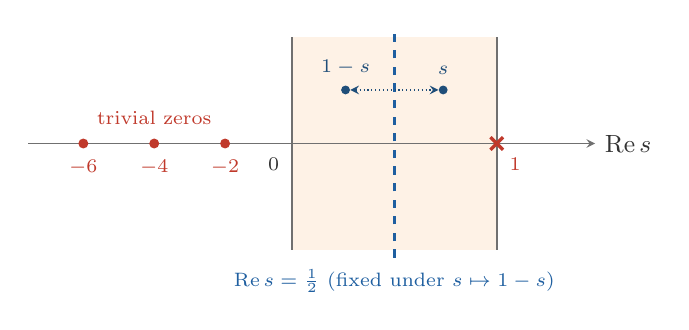
\begin{tikzpicture}[>=stealth,font=\small]
 \fill[lightorange!65] (0,-1.35) rectangle (2.6,1.35);
 \draw[darkgray!70,->] (-3.35,0) -- (3.85,0) node[right,text=darkgray] {$\Real s$};
 \draw[darkgray!70,thick] (0,-1.35) -- (0,1.35);
 \draw[cayleyblue,dashed,very thick] (1.3,-1.45) -- (1.3,1.45);
 \draw[darkgray!70,thick] (2.6,-1.35) -- (2.6,1.35);
 % Trivial zeros at -2, -4, -6
 \foreach \x/\lab in {-0.85/-2, -1.75/-4, -2.65/-6} {
  \fill[cayleyred] (\x,0) circle (1.8pt);
  \node[below,font=\scriptsize,text=cayleyred] at (\x,-0.08) {$\lab$};
 }
 \node[above,font=\scriptsize,text=cayleyred] at (-1.75,0.12) {trivial zeros};
 % Pole at s=1
 \draw[cayleyred,very thick] (2.6-0.08,-0.08) -- (2.6+0.08,0.08);
 \draw[cayleyred,very thick] (2.6-0.08,0.08) -- (2.6+0.08,-0.08);
 % Symmetric pair s and 1-s
 \fill[courseblue] (1.92,0.68) circle (1.6pt) node[above,yshift=2pt,font=\scriptsize,text=courseblue] {$s$};
 \fill[courseblue] (0.68,0.68) circle (1.6pt) node[above,yshift=2pt,font=\scriptsize,text=courseblue] {$1-s$};
 \draw[<->,courseblue,thin,densely dotted] (0.74,0.68) -- (1.86,0.68);
 % Axis labels
 \node[below left,font=\scriptsize,text=darkgray] at (-0.04,-0.06) {$0$};
 \node[below right,font=\scriptsize,text=cayleyred] at (2.64,-0.06) {$1$};
 \node[below,font=\scriptsize,text=cayleyblue] at (1.3,-1.48) {$\Real s=\tfrac12$ (fixed under $s\mapsto 1-s$)};
\end{tikzpicture}

\vspace{0.15em}
{\small Analytic structure of $\zeta(s)$ on $\C$: a unique simple pole at
$s=1$, trivial zeros at $-2,-4,-6,\dots$, and functional-equation symmetry
$s\leftrightarrow 1-s$ across $\Real s=\tfrac12$.}
\end{minipage}
\end{lecturefigure}


% Source: handwritten Lecture 32, Dec. 5, pp. 4--6; Lecture 33, Dec. 7, pp. 1--3.
\section{Nonvanishing of \texorpdfstring{$\zeta(s)$}{zeta(s)} on the line \texorpdfstring{$\Real s = 1$}{Re s = 1}}

We now prove the key analytic fact announced in Lecture~32, which drives
the Prime Number Theorem.

\begin{theorem}[Nonvanishing on $\Real s = 1$]\label{thm:nonvanishing}
The meromorphic continuation of $\zeta(s)$ does not vanish anywhere on the
line $\Real s = 1$; that is, $\zeta(1+it)\neq 0$ for every $t\in\R\setminus\{0\}$.
\end{theorem}

The proof relies on a clever combination of the Euler product and a
trigonometric identity.

\subsection{The logarithm of $\zeta(s)$ for $\Real s > 1$}

Recall from the Euler product (Lecture~32) that
$\zeta(s)=\prod_{p}(1-p^{-s})^{-1}$ for $\Real s > 1$. For any $w\in\C$
with $|w|<1$, the principal branch of the logarithm (branch cut on the
negative real axis) has the power series expansion
\[
 \log\!\left(\frac{1}{1-w}\right) = -\log(1-w) = \sum_{m=1}^{\infty}\frac{w^m}{m}.
\]
Applying this to $w=p^{-s}$ (which has $|p^{-s}|=p^{-\Real s}<1$ for
$\Real s > 1$) motivates defining the series
\begin{equation}\label{eq:log-zeta}
 L(s) = \sum_{p\text{ prime}}\sum_{m=1}^{\infty}\frac{p^{-ms}}{m}
      = \sum_{n=1}^{\infty}\frac{c_n}{n^s}
 \qquad (\Real s > 1),
\end{equation}
where the coefficients $c_n\geq 0$ are supported on prime powers:
\[
 c_n = \begin{cases}
        \dfrac{1}{m} & \text{if } n = p^m \text{ for a prime } p \text{ and } m\geq 1,\\[6pt]
        0 & \text{otherwise.}
       \end{cases}
\]
Since $0\leq c_n\leq 1$ for all $n$, the series \eqref{eq:log-zeta}
converges absolutely for $\Real s > 1$. Moreover, for the first $N$ primes
$p_1,\dots,p_N$,
\[
 \exp\!\left(\sum_{j=1}^{N}\sum_{m=1}^{\infty}\frac{p_j^{-ms}}{m}\right)
 = \prod_{j=1}^{N}\exp\bigl(-\log(1-p_j^{-s})\bigr)
 = \prod_{j=1}^{N}\frac{1}{1-p_j^{-s}}
 \xrightarrow[N\to\infty]{} \zeta(s).
\]
By continuity of the exponential, $e^{L(s)}=\zeta(s)$ for all $\Real s > 1$
(in particular, $\zeta(s)\neq 0$ for $\Real s > 1$, and $L(s)$ is a
holomorphic logarithm $\log\zeta(s)$ on $\{\Real s > 1\}$). Taking absolute
values gives
\[
 |\zeta(s)| = |e^{L(s)}| = e^{\Real L(s)},
 \qquad\text{so}\qquad
 \log|\zeta(s)| = \Real L(s) = \Real\sum_{n=1}^{\infty}\frac{c_n}{n^s}.
\]
Writing $s=\sigma+it$ ($\sigma > 1$, $t\in\R$), we have
\[
 \Real(n^{-s}) = \Real\bigl(e^{-(\sigma+it)\log n}\bigr)
               = e^{-\sigma\log n}\cos(t\log n)
               = n^{-\sigma}\cos(t\log n),
\]
and hence
\begin{equation}\label{eq:log-abs-zeta}
 \log|\zeta(\sigma+it)|
 = \sum_{n=1}^{\infty} c_n n^{-\sigma}\cos(t\log n)
 \qquad (\sigma > 1,\ t\in\R).
\end{equation}

\subsection{The 3--4--1 inequality and proof of Theorem~\ref{thm:nonvanishing}}

\begin{lemma}[The 3--4--1 inequality]\label{lem:341}
For every real $\sigma > 1$ and every $t\in\R$,
\begin{equation}\label{eq:341}
 \boxed{\displaystyle
  \bigl|\zeta(\sigma)^3\,\zeta(\sigma+it)^4\,\zeta(\sigma+2it)\bigr| \geq 1.}
\end{equation}
\end{lemma}

\begin{proof}
Taking logarithms, \eqref{eq:341} is equivalent to
$\log\bigl|\zeta(\sigma)^3\zeta(\sigma+it)^4\zeta(\sigma+2it)\bigr|\geq 0$.
Applying \eqref{eq:log-abs-zeta} at the three points $\sigma$, $\sigma+it$,
and $\sigma+2it$ yields
\begin{align*}
 \log\bigl|\zeta(\sigma)^3\zeta(\sigma+it)^4\zeta(\sigma+2it)\bigr|
 &= 3\log|\zeta(\sigma)| + 4\log|\zeta(\sigma+it)| + \log|\zeta(\sigma+2it)| \\
 &= 3\sum_{n=1}^{\infty} c_n n^{-\sigma}
  + 4\sum_{n=1}^{\infty} c_n n^{-\sigma}\cos(t\log n)
  + \sum_{n=1}^{\infty} c_n n^{-\sigma}\cos(2t\log n) \\
 &= \sum_{n=1}^{\infty} c_n n^{-\sigma}
    \bigl(3 + 4\cos\beta_n + \cos(2\beta_n)\bigr),
\end{align*}
where $\beta_n = t\log n$. By the double-angle identity
$\cos(2\beta)=2\cos^2\beta-1$, every real $\beta$ satisfies
\[
 3 + 4\cos\beta + \cos(2\beta)
 = 3 + 4\cos\beta + (2\cos^2\beta - 1)
 = 2(1+\cos\beta)^2 \geq 0.
\]
Since $c_n\geq 0$ and $n^{-\sigma}>0$ for all $n\geq 1$, every term of the
sum is nonnegative, so
$\log\bigl|\zeta(\sigma)^3\zeta(\sigma+it)^4\zeta(\sigma+2it)\bigr|\geq 0$.
Exponentiating gives \eqref{eq:341}.
\end{proof}

\begin{proof}[Proof of Theorem~\ref{thm:nonvanishing}]
Suppose for contradiction that $\zeta(1+it_0)=0$ for some real $t_0\neq 0$.
We examine each of the three factors in \eqref{eq:341} along the horizontal
rays approaching $1$, $1+it_0$, and $1+2it_0$ as $\sigma\to 1^+$.

\begin{lecturefigure}
\begin{minipage}{\linewidth}\centering
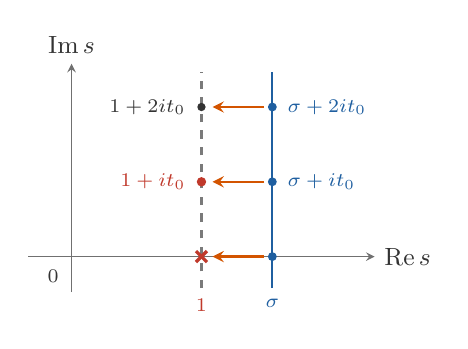
\begin{tikzpicture}[>=stealth,font=\small]
 \draw[darkgray!70,->] (-0.55,0) -- (3.85,0) node[right,text=darkgray] {$\Real s$};
 \draw[darkgray!70,->] (0,-0.45) -- (0,2.45) node[above,text=darkgray] {$\Imag s$};
 \draw[darkgray!65,dashed,thick] (1.65,-0.4) -- (1.65,2.35);
 \draw[cayleyblue,thick] (2.55,-0.4) -- (2.55,2.35);
 % Points on Re s = 1
 \draw[cayleyred,very thick] (1.65-0.07,-0.07) -- (1.65+0.07,0.07);
 \draw[cayleyred,very thick] (1.65-0.07,0.07) -- (1.65+0.07,-0.07);
 \fill[cayleyred] (1.65,0.95) circle (1.7pt);
 \fill[darkgray] (1.65,1.90) circle (1.5pt);
 % Points on Re s = sigma and arrows to Re s = 1
 \foreach \y/\lab in {0/\sigma, 0.95/\sigma+it_0, 1.90/\sigma+2it_0} {
  \fill[cayleyblue] (2.55,\y) circle (1.6pt);
  \draw[->,cayleyorange,thick,shorten <=3pt,shorten >=4pt] (2.55,\y) -- (1.65,\y);
 }
 \node[below left,font=\scriptsize,text=darkgray] at (-0.04,-0.05) {$0$};
 \node[below,font=\scriptsize,text=cayleyred] at (1.65,-0.42) {$1$};
 \node[below,font=\scriptsize,text=cayleyblue] at (2.55,-0.42) {$\sigma$};
 \node[left,font=\scriptsize,text=cayleyred] at (1.57,0.95) {$1+it_0$};
 \node[left,font=\scriptsize,text=darkgray] at (1.57,1.90) {$1+2it_0$};
 \node[right,font=\scriptsize,text=cayleyblue] at (2.62,0.95) {$\sigma+it_0$};
 \node[right,font=\scriptsize,text=cayleyblue] at (2.62,1.90) {$\sigma+2it_0$};
\end{tikzpicture}

\vspace{0.15em}
{\small Letting $\sigma\to 1^+$ drives the three points $\sigma$,
$\sigma+it_0$, and $\sigma+2it_0$ toward the pole $1$, the putative zero
$1+it_0$, and the regular point $1+2it_0$.}
\end{minipage}
\end{lecturefigure}

\begin{enumerate}[label=\textup{(\arabic*)}]
 \item \textbf{Near $1+it_0$:} Since $\zeta$ is holomorphic at $1+it_0$ and
       vanishes there (with order $k\geq 1$), its Taylor expansion near
       $z_0=1+it_0$ has the form
       $\zeta(z)=c(z-z_0)^k\bigl(1+a_1(z-z_0)+\cdots\bigr)$. Thus there is
       a constant $C>0$ such that for $\sigma>1$ sufficiently close to $1$,
       \[
        |\zeta(\sigma+it_0)| \leq C(\sigma-1),
        \qquad\text{so}\qquad
        |\zeta(\sigma+it_0)|^4 \leq C^4(\sigma-1)^4.
       \]
 \item \textbf{Near $s=1$:} Since $\zeta$ has a simple pole at $s=1$,
       $(s-1)\zeta(s)$ is holomorphic near $s=1$, so there is a constant
       $C'>0$ such that for $\sigma>1$ sufficiently close to $1$,
       \[
        |\zeta(\sigma)| \leq \frac{C'}{\sigma-1},
        \qquad\text{so}\qquad
        |\zeta(\sigma)|^3 \leq \frac{(C')^3}{(\sigma-1)^3}.
       \]
 \item \textbf{Near $1+2it_0$:} Since $t_0\neq 0$, we have $1+2it_0\neq 1$,
       so $\zeta$ is holomorphic (hence bounded) near $1+2it_0$: there is
       a constant $B>0$ such that $|\zeta(\sigma+2it_0)|\leq B$ for
       $\sigma>1$ sufficiently close to $1$.
\end{enumerate}

Combining these three estimates with Lemma~\ref{lem:341} gives, for
$\sigma>1$ sufficiently close to $1$,
\[
 1 \leq \bigl|\zeta(\sigma)^3\,\zeta(\sigma+it_0)^4\,\zeta(\sigma+2it_0)\bigr|
   \leq \frac{(C')^3}{(\sigma-1)^3}\cdot C^4(\sigma-1)^4\cdot B
   = B C^4 (C')^3\,(\sigma-1) \xrightarrow[\sigma\to 1^+]{} 0,
\]
a contradiction! Therefore $\zeta(1+it_0)\neq 0$ for all $t_0\neq 0$.
\end{proof}


% Source: handwritten Lecture 33, Dec. 7, pp. 3--5.
\section{Toward the Prime Number Theorem: Chebyshev's function}

We close the course by introducing the prime-counting machinery used to
pass from Theorem~\ref{thm:nonvanishing} to the Prime Number Theorem
$\pi(x)\sim x/\log x$.

\begin{definition}[Asymptotic notation]
Let $f$ and $g$ be functions defined for sufficiently large real $x$.
\begin{itemize}
 \item We write $f(x)\sim g(x)$ (as $x\to\infty$) if
       $\displaystyle\lim_{x\to\infty}\frac{f(x)}{g(x)}=1$.
 \item For $f(x)>0$, we write $g(x)=O(f(x))$ if there exist constants
       $C>0$ and $x_0$ such that $|g(x)|\leq C f(x)$ for all $x\geq x_0$.
       For example, $g(x)=O(1)$ means $g$ is bounded for large $x$.
\end{itemize}
\end{definition}

Rather than counting primes directly via $\pi(x)=\#\{p\leq x\}$, it is
often cleaner to weight each prime $p$ by $\log p$.

\begin{definition}[Chebyshev's prime-counting function]
For $x>0$, define
\[
 \psi(x) = \sum_{p\leq x} \log p,
\]
where the sum runs over all prime numbers $p\leq x$ (with $\psi(x)=0$ for
$x<2$).
\end{definition}

\begin{lemma}[Chebyshev's upper bound]\label{lem:chebyshev}
$\psi(x) = O(x)$ as $x\to\infty$; that is, there is a constant $C'>0$ such
that $\psi(x)\leq C'x$ for all $x\geq 1$.
\end{lemma}

The heart of the proof is an elementary divisibility observation for the
central binomial coefficient $\binom{2n}{n}$.

\begin{exercise}[Primes dividing $\binom{2n}{n}$]\label{ex:central-binom}
For any integer $n\geq 1$, write
\[
 \binom{2n}{n} = \frac{(2n)!}{n!\,n!} = \frac{(2n)(2n-1)\cdots(n+1)}{n!}.
\]
Show that every prime $p$ satisfying $n < p \leq 2n$ divides $\binom{2n}{n}$,
and deduce that
\[
 \binom{2n}{n} \geq \prod_{n < p \leq 2n} p.
\]
\emph{Hint:} Since $p > n$, $p$ divides the numerator $(2n)\cdots(n+1)$ but
does not divide $n!$; distinct primes are pairwise coprime.
\end{exercise}

\begin{proof}[Proof of Lemma~\ref{lem:chebyshev}]
\textbf{Step 1: Bound at integers $n\geq 1$.}
By the binomial theorem,
\[
 2^{2n} = (1+1)^{2n} = \binom{2n}{0} + \binom{2n}{1} + \cdots + \binom{2n}{2n}
 \geq \binom{2n}{n}.
\]
On the other hand, since $e^{\psi(x)}=\exp\bigl(\sum_{p\leq x}\log p\bigr)=\prod_{p\leq x} p$,
Exercise~\ref{ex:central-binom} gives
\[
 e^{\psi(2n)-\psi(n)} = \prod_{n < p \leq 2n} p \leq \binom{2n}{n} \leq 2^{2n}.
\]
That is,
\begin{equation}\label{eq:psi-int}
 \boxed{\displaystyle e^{\psi(2n)-\psi(n)} \leq 2^{2n},}
 \qquad\text{so}\qquad
 \psi(2n)-\psi(n) \leq (2\log 2)\,n.
\end{equation}

\textbf{Step 2: Extension to all real $x\geq 1$.}
Whenever $x$ increases by $1$, at most one integer in $(x,x+1]$ can be
prime, so $\psi(x)$ increases by at most $\log(x+1)=O(\log x)$.

More concretely, take any real $x\geq 2$ and set $n=\lfloor x/2\rfloor\geq 1$.
Then $n\leq x/2 < n+1$, so $2n\leq x < 2n+2$. Because $2n+2>2$ is even,
the only integer in $(2n,x]$ that can be prime is $2n+1$ (which occurs only
when $2n+1\leq x$). Hence $\psi(x)-\psi(2n)\leq \log x$, and combining this
with \eqref{eq:psi-int} and $\psi(x/2)\geq\psi(n)$ gives
\[
 \psi(x)-\psi(x/2)
 \leq \bigl(\psi(2n)-\psi(n)\bigr) + \bigl(\psi(x)-\psi(2n)\bigr)
 \leq (2\log 2)\,n + \log x
 \leq (\log 2)\,x + \log x.
\]
Since $\log x\leq x$ for all $x\geq 1$, setting $C=1+\log 2$ gives
\begin{equation}\label{eq:psi-dyadic}
 \boxed{\displaystyle \psi(x) - \psi(x/2) \leq C x}
\end{equation}
for all $x\geq 2$ (and trivially for $1\leq x < 2$, where both sides are
$0\leq Cx$).

\textbf{Step 3: Telescoping dyadic sum.}
For any $x\geq 1$, choose an integer $r\geq 1$ such that $x/2^r < 2$ (so
$\psi(x/2^r)=0$). Summing \eqref{eq:psi-dyadic} over the dyadic points
$x,\,x/2,\,x/4,\,\dots,\,x/2^{r-1}$ telescopes:
\begin{align*}
 \psi(x)
 &= \bigl(\psi(x)-\psi(x/2)\bigr)
  + \bigl(\psi(x/2)-\psi(x/4)\bigr)
  + \cdots
  + \bigl(\psi(x/2^{r-1})-\psi(x/2^r)\bigr) \\
 &\leq C\left(x + \frac{x}{2} + \frac{x}{4} + \cdots + \frac{x}{2^{r-1}}\right)
  < C x \sum_{k=0}^{\infty}\frac{1}{2^k} = 2C x.
\end{align*}
Setting $C'=2C$ gives $\psi(x)\leq C'x$ for all $x\geq 1$, so $\psi(x)=O(x)$.
\end{proof}

\textbf{From $\psi(x)=O(x)$ and $\zeta(1+it)\neq 0$ to the Prime Number Theorem.}
With $\psi(x)=O(x)$ in hand, the Laplace/Mellin transform
$\Phi(s)=\sum_{p}\frac{\log p}{p^s}=s\int_1^{\infty}\frac{\psi(x)}{x^{s+1}}\,dx$
connects $\psi(x)$ directly to $-\zeta'(s)/\zeta(s)$ (via the Euler
product). Because $\zeta(s)$ extends meromorphically with a simple pole at
$s=1$ and no zeros on $\Real s = 1$ (Theorem~\ref{thm:nonvanishing}),
$\Phi(s)-\frac{1}{s-1}$ extends holomorphically to a neighborhood of the
closed half-plane $\{\Real s \geq 1\}$. Using Cauchy's theorem on a
contour crossing slightly to the left of $\Real s = 1$ (Newman's analytic
theorem), one obtains the main analytic fact:
\begin{equation}\label{eq:main-analytic-fact}
 \boxed{\displaystyle
  \int_1^{\infty}\frac{\psi(x)-x}{x^2}\,dx < \infty}
 \qquad\text{(i.e., the improper integral converges).}
\end{equation}

\begin{remark}[Completing the Prime Number Theorem]
Once \eqref{eq:main-analytic-fact} is established, two elementary
real-variable arguments finish the Prime Number Theorem:
\begin{enumerate}[label=\textup{(\arabic*)}]
 \item Because $\psi(x)$ is nondecreasing, the convergence of
       $\int_1^{\infty}\frac{\psi(x)-x}{x^2}\,dx$ forces $\psi(x)\sim x$
       as $x\to\infty$ (if $\psi(x)\geq(1+\delta)x$ at arbitrarily large
       $x$, monotonicity would force $\psi(t)-t$ to stay large on
       $[x,(1+\delta)x]$, making the tail integral bounded below by a
       positive constant; similarly for $\psi(x)\leq(1-\delta)x$).
 \item The asymptotic $\psi(x)\sim x$ is easily seen to be equivalent to
       the Prime Number Theorem $\pi(x)\sim x/\log x$: on the one hand
       $\psi(x)=\sum_{p\leq x}\log p\leq\pi(x)\log x$; on the other hand,
       for any $0<\varepsilon<1$,
       $\psi(x)\geq\sum_{x^{1-\varepsilon}<p\leq x}\log p\geq(1-\varepsilon)(\log x)\bigl(\pi(x)-x^{1-\varepsilon}\bigr)$,
       which forces $\frac{\pi(x)}{x/\log x}\to 1$ as $x\to\infty$.
\end{enumerate}
\end{remark}

\end{document}
